\chapter{Testing and practical application of text classification using software} \label{chapt3}
\section{Software selection} \label{sect3_1}

The most popular languages in data analysis area are Python and R.
Python3 language was chosen as more convenient for machine learning and beyond variety of libraries, including:

\begin{itemize}
	\item pandas
	\item sklearn
	\item gensim
	\item keras
	\item tensorflow
	\item matplotlib
	\item psycopg2
\end{itemize}

The prototyping of models were made in the separate Jupyter notebooks and then re-factored into 
project using the Python IDE for developers be JetBrains company - PyCharm. 
The server with  Intel(R) Core(TM) i7-4770 CPU @ 3.40GHz, 15 $\times$ 2 GB DDR3-1333 was used. 

As a word vectors representation I used pre-trained word vectors which were trained on Wikipedia using fastText technique by Facebook research team and shared to the community \cite{fasttext}. These vectors in dimension 300 were obtained using the skip-gram model with default parameters.

My main requirement for the framework for building deep neural network models were:
\begin{itemize}
	\item well described documentation
	\item simplicity of usage
	\item learning speed
	\item reliability
\end{itemize}

Among a wide range of frameworks which are available in open source: 
CNTK, Theano, MAXNET, Lasagne - Tensorflow framework was chosen. 
Tensorflow has a flexible architecture allows easy deployment of computation across a variety of platforms (CPUs, GPUs, TPUs). To speed up the experiments with architecture of NN, I switched to a high-level neural networks API, written in Python and capable of running on top of TensorFlow. 

\section{Dataset selection and exploration} \label{sect3_2}

The target attribute to be predicted is the category of the advertisements. The category is represented by the two-level hierarchy. The parent category consists 16 categories which then branches into 183 subcategories. These categories can be mapped together in the following way:

\begin{table}[h]
	\centering
	\caption{The hierarchy of categories}
	\label{my-label}
	\begin{tabular}{|c|c|}
		\hline
		\textbf{lvl2}      & category ID     \\
		\hline
		\textbf{lvl1}	 		  & identifier of the parent category		 \\
		\hline
		\textbf{name}	 		  & category name		 \\
		\hline
	\end{tabular}
\end{table}

The dataset contains 455,000 ads classified into 183 categories. 
The sample of dataset can be seen from the Table \ref{data_structure}.
First, let us get familiar with data and how it distributes between categories.
As it can be clearly seen from the Table \ref{general} we have 2 categorical 
and 2 numerical variables and our data does not have any missing fields. 
That is good to start examine our data by each variable separately. 
From Table \ref{lvl1} we can see that data is not distributed equally between 
categories. First level categories with number \textbf{6,5,1} consist almost a half 
of all advertisements. That means that our data is imbalanced and we can not 
use accuracy as only one metric for evaluation. 
Then if we take a look at second level categories Table \ref{lvl2} we will see even worst picture: one third of the date is concentrated in the categories which are marked \textbf{29,14} and \textbf{55} respectively. 
That means that it is necessary to use techniques to regularize distributions: under/over sampling or weight balanced.

For evaluation such metrics as categorical\_accuracy
, categorical\_crossentropy, loss, timing and top\_k\_categorical\_accuracy were chosen. 


\begin{table}[]
	\centering
	\caption{Structure of the data files}
	\label{data_structure}
	\begin{tabular}{| p{1cm} | p{1cm} | p{3cm} | p{7cm} |}
		\hline
		\textbf{lvl1} & \textbf{lvl2} & \textbf{titles}                  & \textbf{descriptions}                                                                       \\ \hline
		6             & 29            & Clean Toyota Camry 2008 Silver   & Fairly used Toyota 08 Camry with no problems V4 engine fabric seats and interior            \\ \hline
		5             & 25            & Look Unique                      & Nice, quality, adorable,unique dress available now, whatsapp me                             \\ \hline
		6             & 29            & Mercedes Benz Ml 430 2001 Silver & mercedes benz ml430 , 2001 model in good condition , engine and gear box ok, ac , cd player \\ \hline
		5             & 25            & Versace Shirt Dress              & Adorable versace shirt dress, whatsapp me on \_large\_number\_                              \\ \hline
		5             & 25            & Addidas Jumpsuit                 & Nice quality addidas jumpsuit available, whatsapp me                                        \\ \hline
	\end{tabular}
\end{table}


\begin{table}[h]
	\centering
	\caption{Training set general information}
	\label{general}
	\begin{tabular}{|c|c|}
		\hline
	\textbf{	Number of variables     }      & 4      \\
		\hline
	\textbf{	Numeric variables}	 		  & 2		 \\
		\hline
	\textbf{	Categorical	variables} 		  & 2		 \\
		\hline
		\textbf{Number of observations }       & 455000  \\
		\hline
		\textbf{Total Missing (\%) }           & 0.0\%    \\
		\hline
		\textbf{Total size in memory }         & 57.7 MiB \\
		\hline
		\textbf{Average record size in memory} & 48.0 B  \\
		\hline
	\end{tabular}
\end{table}


\begin{table}[h]
	\centering
	\caption{Information about first level categories}
	\label{lvl1}
	\begin{tabular}{|l|l|l|l|}
		\hline
	\textbf{Value }             & \textbf{Count}  & \textbf{Frequency} (\%) \\ \hline
		6                & 207695 & 20.8\%           \\ \hline
		5                & 184934 & 18.5\%           \\ \hline
		1                & 133135 & 13.3\%           \\ \hline
		4                & 97799  & 9.8\%            \\ \hline
		3                & 87574  & 8.8\%           \\ \hline
		110              & 60214  & 6.0\%            \\ \hline
		9                & 55459  & 5.5\%            \\ \hline
		27               & 52419  & 5.2\%            \\ \hline
		47               & 38985  & 3.9\%            \\ \hline
		140              & 36442  & 3.6\%           \\ \hline
		Other values (6) & 45344  & 4.5\%            \\ \hline
	\end{tabular}
\end{table}


\begin{table}[h]
	\centering
	\caption{Information about second level categories}
	\label{my-label}
	\begin{tabular}{|l|l|l|}
		\hline
		\textbf{Value }             & \textbf{Count}  & \textbf{Frequency} (\%) \\ \hline
		29                 & 194714 & 19.5\%         \\ \hline
		14                 & 115471 & 11.5\%         \\ \hline
		55                 & 72050  & 7.2\%          \\ \hline
		25                 & 61308  & 6.1\%          \\ \hline
		16                 & 32719  & 3.3\%          \\ \hline
		20                 & 23298  & 2.3\%          \\ \hline
		169                & 18743  & 1.9\%          \\ \hline
		42                 & 18490  & 1.8\%          \\ \hline
		44                 & 17740  & 1.8\%          \\ \hline
		279                & 15544  & 1.6\%          \\ \hline
		Other values (172) & 429923 & 43.0\%         \\ \hline
	\end{tabular}
\end{table}


\begin{table}[h]
	\centering
	\caption{Information about categorical features}
	\label{my-label}
	\begin{tabular}{llll}
		\hline
\multicolumn{1}{|l|}{\textbf{Column}} & \multicolumn{1}{l|}{\textbf{Distinct count}} & \multicolumn{1}{l|}{\textbf{Unique (\%)}} & \multicolumn{1}{l|}{\textbf{Missing (\%)}} \\ \hline
		\multicolumn{1}{|l|}{titles}       & \multicolumn{1}{l|}{619948}         & \multicolumn{1}{l|}{62.0\%}      & \multicolumn{1}{l|}{0.00\%}       \\ \hline
		\multicolumn{1}{|l|}{descriptions} & \multicolumn{1}{l|}{869554}         & \multicolumn{1}{l|}{87.0\%}      & \multicolumn{1}{l|}{0.00\%}       \\ \hline
	\end{tabular}
\end{table}


I decided to divide the whole dataset into train.csv / test.csv files which have the following structure:training set contains 400000 observation and control sample - 55,000 ads. 

\clearpage
\section{Data preparation} \label{sect3_3}

\begin{figure}[ht] 
	\center
	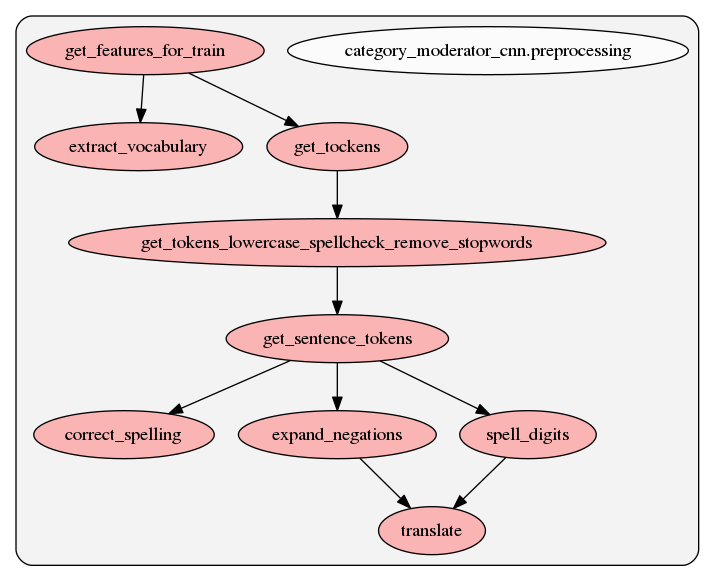
\includegraphics [scale=0.5] {p3_preprocessing.png}
	\label{img:p3_preprocessing}  
	\caption{Simplified event structure of data preprocessing} 
\end{figure}


\noindent \textbf{1.Tokenize Text}

The given text was split by spaces and then lemmatized.

\noindent \textbf{2. Remove infrequent words}

Words which appears less than 3 times in the whole corpus were removed. It’s a good idea to remove these infrequent words because a huge vocabulary will make our model slow to train and not all these words are presented in pretrained embeddings. 
Special attention should be paid numbers which can be represented as price, year, mobile number. The telephone numbers occur really frequently in advertisements, but in most cases, they are unique because different people have their own telephone numbers - the information about whether a telephone number presents in text or not is meaningful. I used regular expressions to replace all numbers with the words \_large\_number\_, \_small\_num\_,  \_price\_, \_year\_. which gave me a possibility not to lose precious information. 
\\

\noindent
\textit{\textbf{r'[0-9a-z\_]+@[a-z]+\.[a-z]+': '\_email\_', \\
r'[0-9]{5,20}': '\_large\_number\_',\\
r'[1-9][0-9]*k': '\_price\_',
\\
r'[1-9][0-9]+?,[0-9]*': '\_price\_',
\\
r'[1-9][0-9]*?,[0-9]* thousand': '\_price\_',
\\
r'19[0-9]{2}': '\_year\_',
\\
r'200[0-9]': '\_year\_',
\\
r'201[0-8]': '\_year\_',
\\
r'[0-9]+': '\_small\_num\_',}}
\\

\noindent \textbf{3. Correct misspellings}

I analyzed properly the most frequent cases where users do mistakes. Then I created a dictionary which consists wrong and right written words, so each time when the wrong written word appears it is replaced with the right written equivalent. 

\newcolumntype{b}{X}
\newcolumntype{s}{>{\hsize=.5\hsize}X}

\begin{table}[h]
	\centering
	\caption{Simplified event structure of data preprocessing}
	\label{my-label}
	\begin{tabular}{| p{7cm} | p{10cm} |}
%	\begin{tabulary}{1.0\textwidth}{|L|L|L|L|L|L}
		\hline
		\textbf{Functions}                                    & \textbf{Explanation}                                                                                                                \\ \hline
		get\_features\_for\_train                             & unifying function which upload raw data and call nested functions                                                                   \\ \hline
		extract\_vocabulary                                   & form vocabulary from unique words                                                                                                   \\ \hline
		get\_tokens                                           & parallel batch execution of texts preprocessing which save and return preprocessed tokens for both test and train.                  \\ \hline
		get\_tokens\_lowercase\_spellcheck\ & wrap over get\_sentence\_tokens which set necessary flags for it                                                                    \\ \hline
		get\_sentence\_tokens                                 & recieves single sentence breaks it into tokens, make all of them to lowercase, correct spelling mistakes and replace specific words \\ \hline
		correct\_spelling                                     & correct spelling mistakes using dictionary with around 15000 most common mistakes                                                   \\ \hline
		expand\_negations                                     & replace mobile phones, dates, prices, and common abbreviation with specific words such as \_year\_, price,  \_large\_number\_ etc.  \\ \hline
		spell\_digits                                         & single digits are replaced with corresponding word 1 $\rightarrow$ one …                                                                          \\ \hline
		translate                                             & function which makes replacement of words                                                                                           \\ \hline
	\end{tabular}
\end{table}



\noindent \textbf{4. Build embeddings }

\begin{figure}[ht] 
	\center
	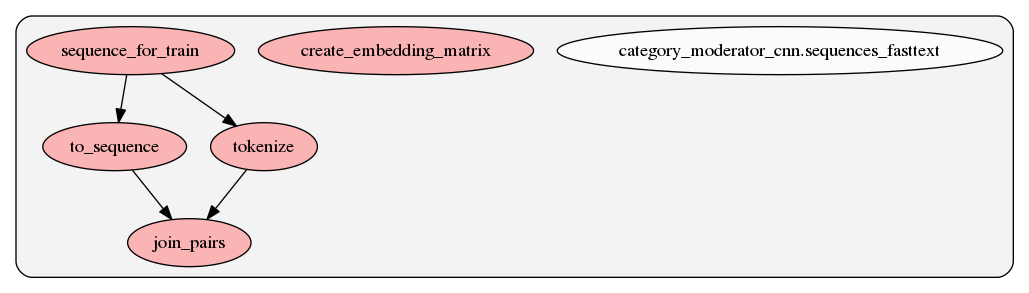
\includegraphics [scale=0.45] {p3_sequences_fasttext.png}
	\label{img:p3_sequences_fasttext}  
	\caption{Build embeddings structure} 
\end{figure}


The input to Neural Networks are vectors, not strings. The mapping between words and indices was created, index\_to\_word, and word\_to\_index. For example,  the word “buy” may be at index 201. 



\begin{table}[h]
	\centering
	\caption{Simplified event structure of data preprocessing}
	\label{my-label}
	\begin{tabular}{| p{7cm} | p{10cm} |}
		%	\begin{tabulary}{1.0\textwidth}{|L|L|L|L|L|L}
		\hline
		\textbf{Functions}                                    & \textbf{Explanation}                                                                                                                \\ \hline
		sequence\_for\_train                             & loads preprocessed tokens from previous model and use functions listed below to create sequence of indices which corresponds to particular word.                                                                    
		\\ \hline
		to\_sequence                                   & encode each word with the corresponding index        and organize them into sequences of indices with the particular length                                                      \\ \hline
		tokenize                                           & build and save tokenizer which maps words and their indices 
		\\ \hline
		join\_pairs &  helpful function for transformation                                                      
		\\ \hline
		create\_embedding\_matrix                                 & build the embedding matrix for unique words from our dataset. It will have the structure word represented by it index in our vocabulary and the corresponding vector from the pre-trained embedding model. \\ \hline

	\end{tabular}
\end{table}





\clearpage
\section{Network design and training} \label{sect3_4}


\begin{figure}[ht] 
	\center
	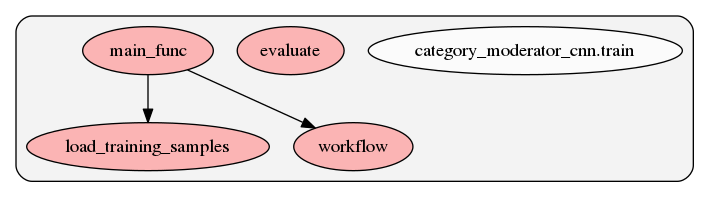
\includegraphics [scale=0.5] {p3_train.png}
	\label{img:p3_train}  
	\caption{4} 
\end{figure}


In this module I implemented different types of neural networks. Each network design module describe only
one type of networks, that makes text classification. After the design of NN was implemented it should be trained. Apart from the training part this module saves training statistics \ref{img:p3_custom_callbacks} such as: 
\begin{itemize}
	\item categorical accuracy
	\item top k categorical accuracy
	\item batch timer
	\item categorical loss
	\item histograms of NN weights
\end{itemize}

These metrics will be used to judge the performance of our model. 
Such statistics give more information about changes in neural network on each step of training. 
As tested network types on this step, I choose bidirectional recurrent network 
and convolutional network with different window sizes. 


\begin{figure}[ht] 
	\center
	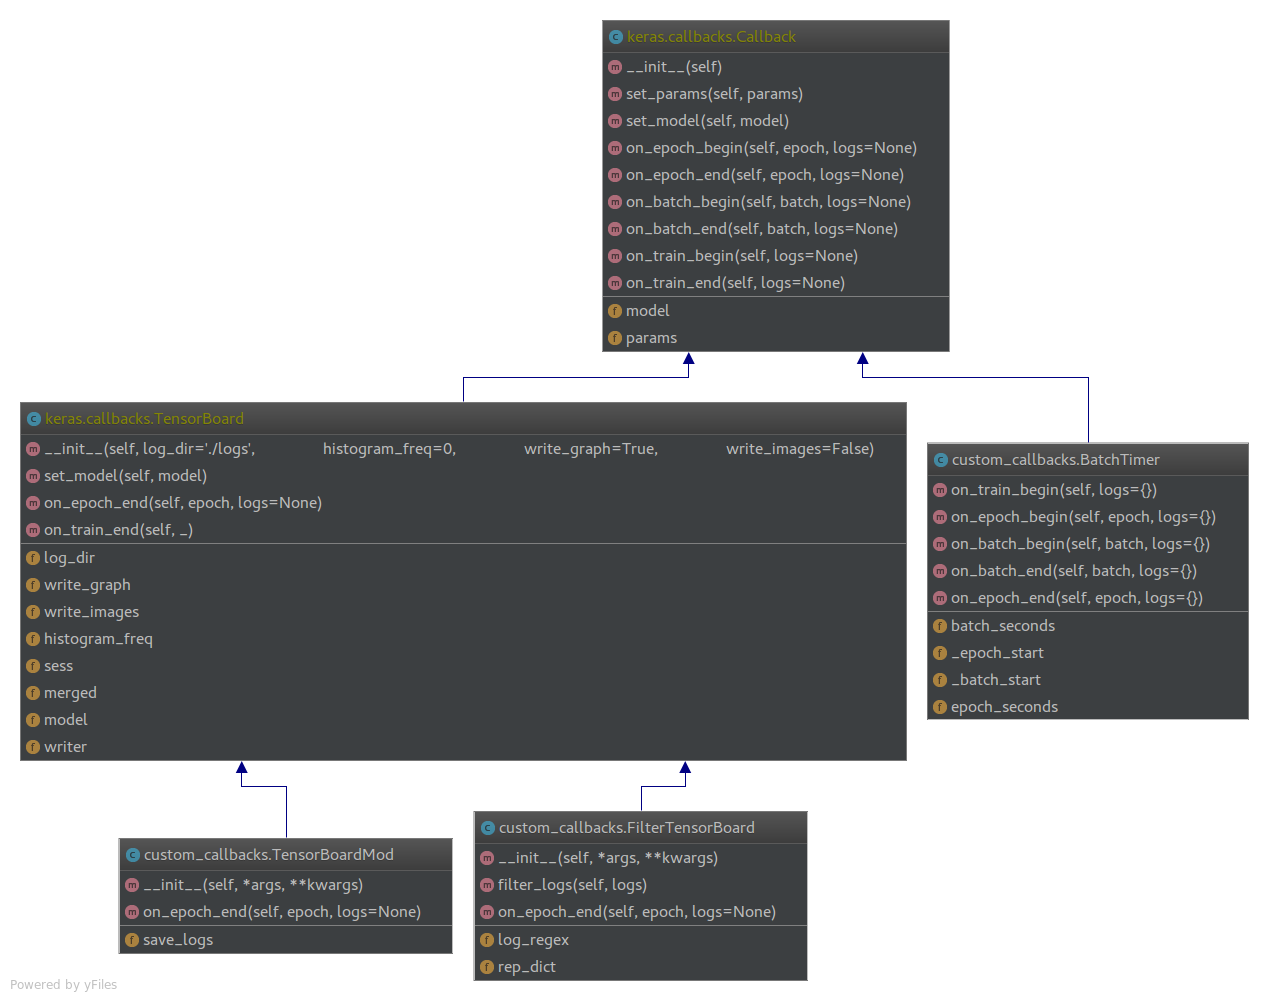
\includegraphics [scale=0.25] {p3_custom_callbacks.png}
	\label{img:p3_custom_callbacks}  
	\caption{Metrics which were logged} 
\end{figure}

\clearpage
\section{Summary of the section}\label{sect3_5}
This section argue the usage of the selected software. The detailed analysis of the data was provided. 
Also, we went through the implementation process as well: from the raw data to the trained model.
The explanation of the most significant functions was made. 
